% -*- coding: utf-8 -*-

% This LaTeX was auto-generated from an M-file by MATLAB.
% To make changes, update the M-file and republish this document.

\documentclass{article}
\usepackage{graphicx}
\usepackage{color}

% ++++++++++++ attach the following code
% 2010-4-16 10:56上午,添加中文支持模块

\usepackage{xeCJK}
\setCJKmainfont{FangSong_GB2312}
% ++++++++++++ finish attaching

\sloppy
\definecolor{lightgray}{gray}{0.5}
\setlength{\parindent}{0pt}

\begin{document}

    
    \begin{verbatim}
% 2010-4-15, luyz23, 从MATLAB到latex的简单示例
% >> publish('kalmanfilter.m','latex')
% -*-  卡尔曼滤波 -*-
% 此范例源自:网络论坛,在此感谢
clear
N=800; w(1)=0; w=randn(1,N); %系统预测的随机白噪声
x(1)=0; a=1;
for k=2:N;
    x(k)=a*x(k-1)+w(k-1); %系统的预测值
end
V=randn(1,N); %测量值的随机白噪声
q1=std(V); Rvv=q1.^2;
q2=std(x); Rxx=q2.^2;
q3=std(w); Rww=q3.^2;
c=0.2;
Y=c*x+V; %测量值
p(1)=0; s(1)=0;
for t=2:N;
    p1(t)=a.^2*p(t-1)+Rww; %前一时刻X的相关系数
    b(t)=c*p1(t)/(c.^2*p1(t)+Rvv); %卡尔曼增益
    s(t)=a*s(t-1)+b(t)*(Y(t)-a*c*s(t-1)); %经过滤波后的信号
    p(t)=p1(t)-c*b(t)*p1(t);%t状态下x(t|t)的相关系数
end
figure(1); plot(x); title('系统的预测值')
figure(2); plot(Y); title('测量值')
figure(3); plot(s); title('滤波后的信号')
\end{verbatim}

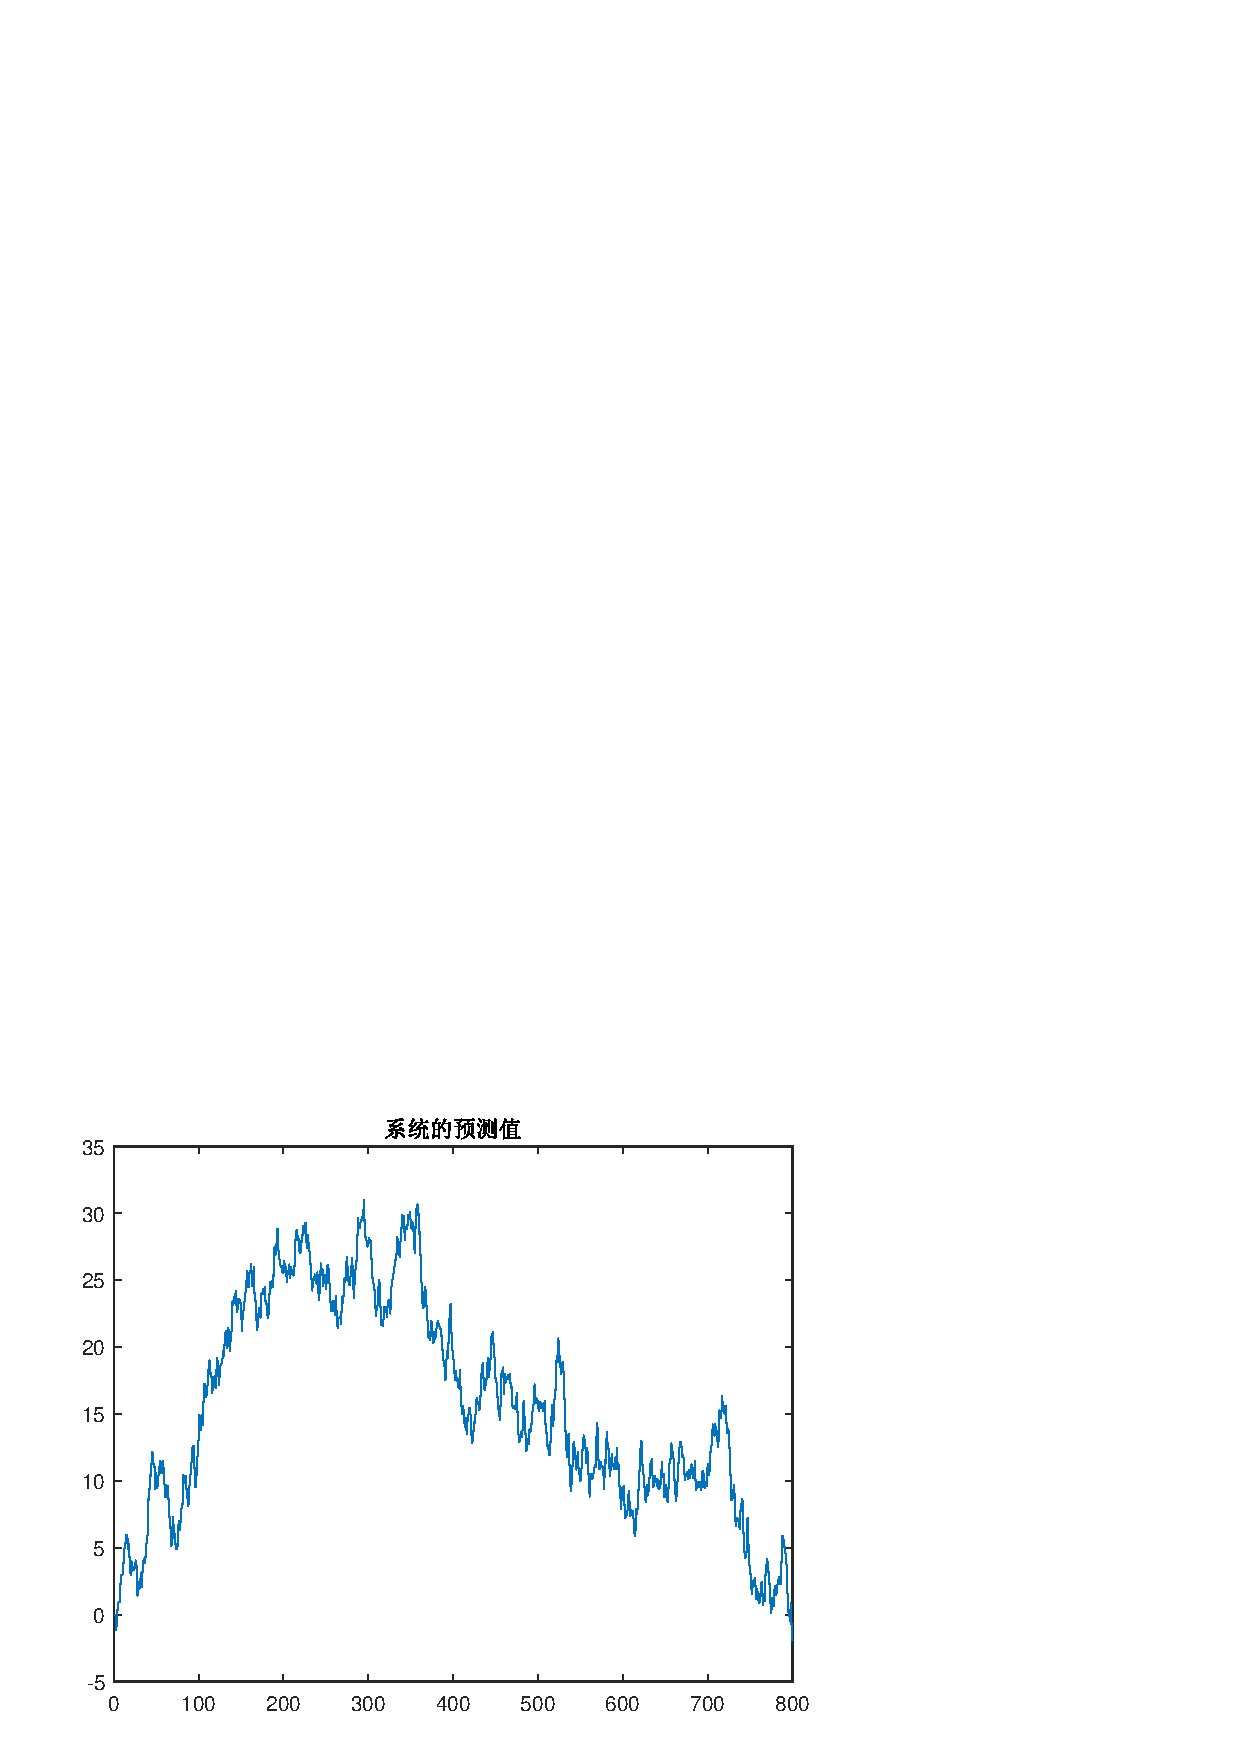
\includegraphics [width=4in]{kalmanfilter_01.png}\\

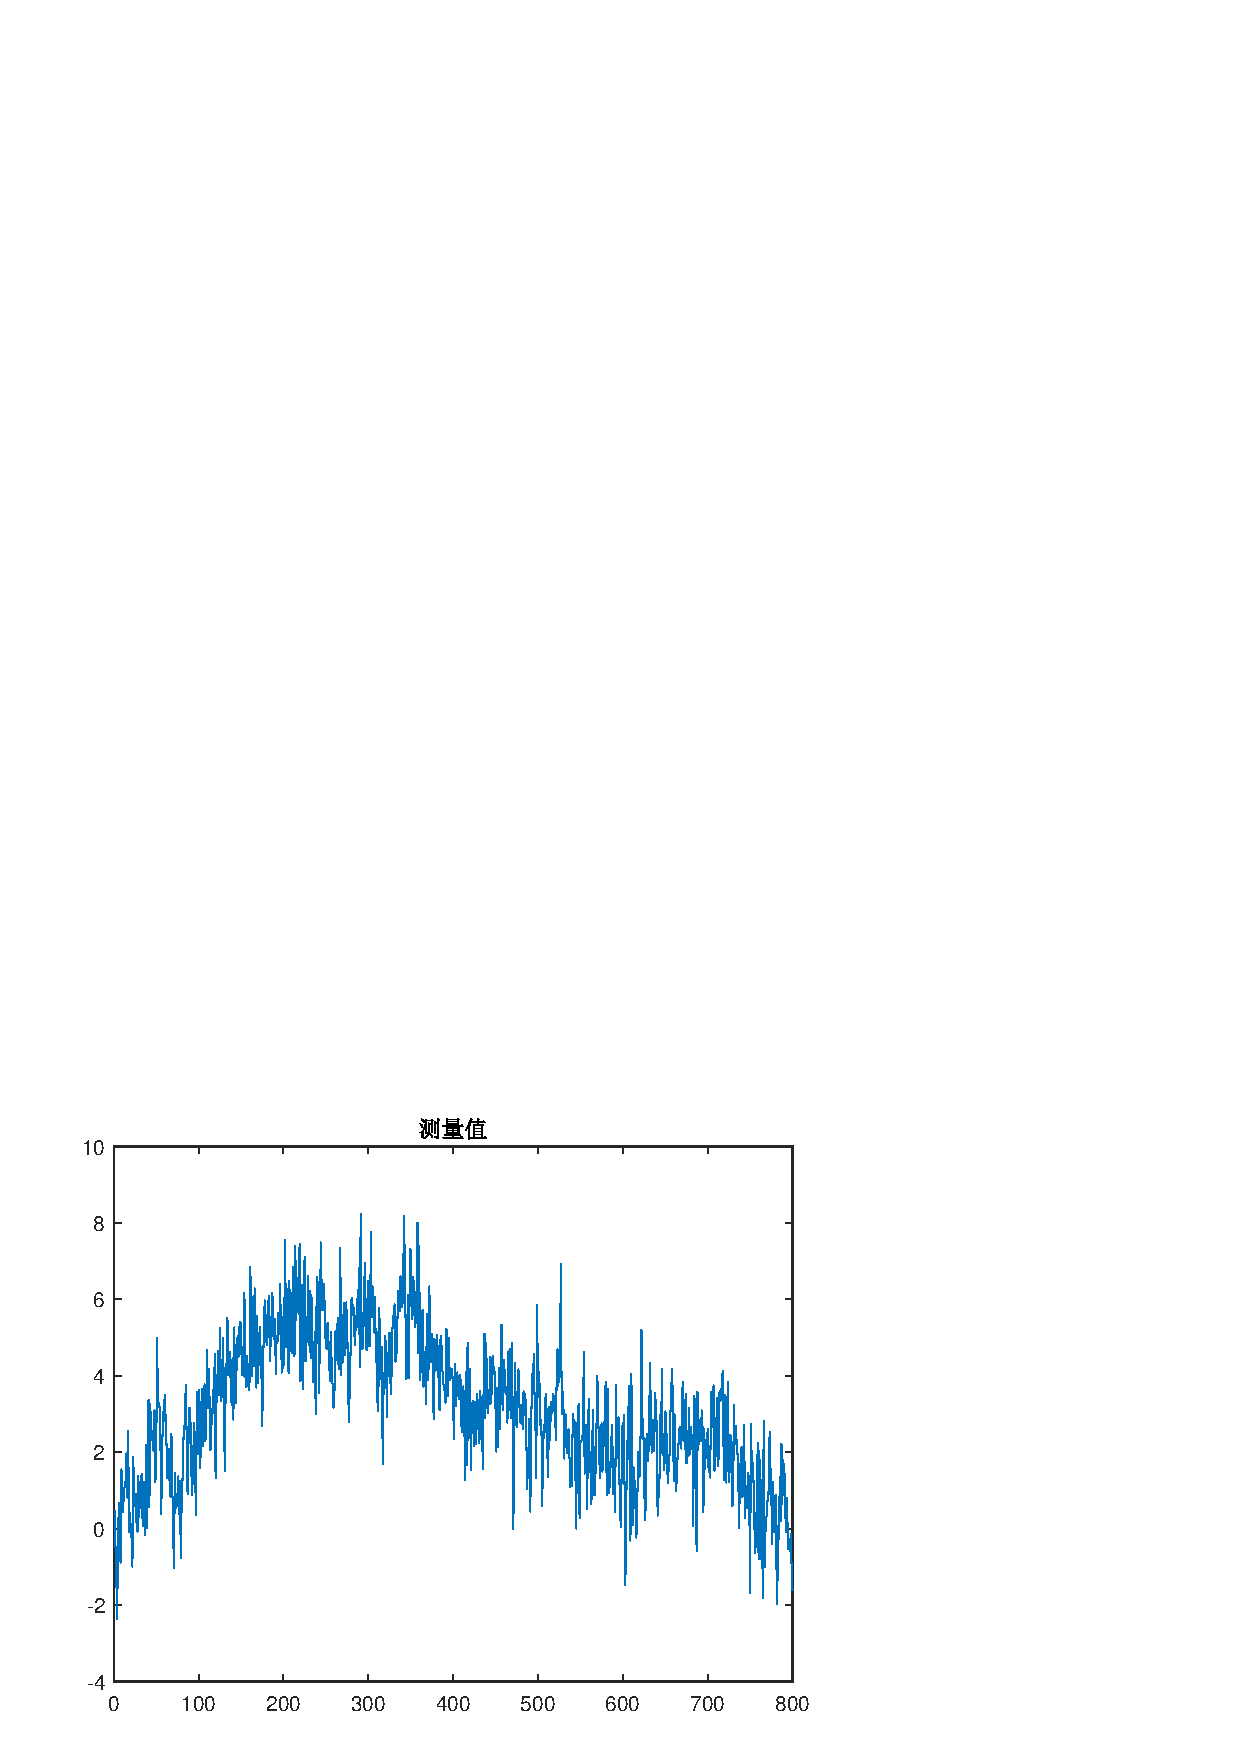
\includegraphics [width=4in]{kalmanfilter_02.png}\\

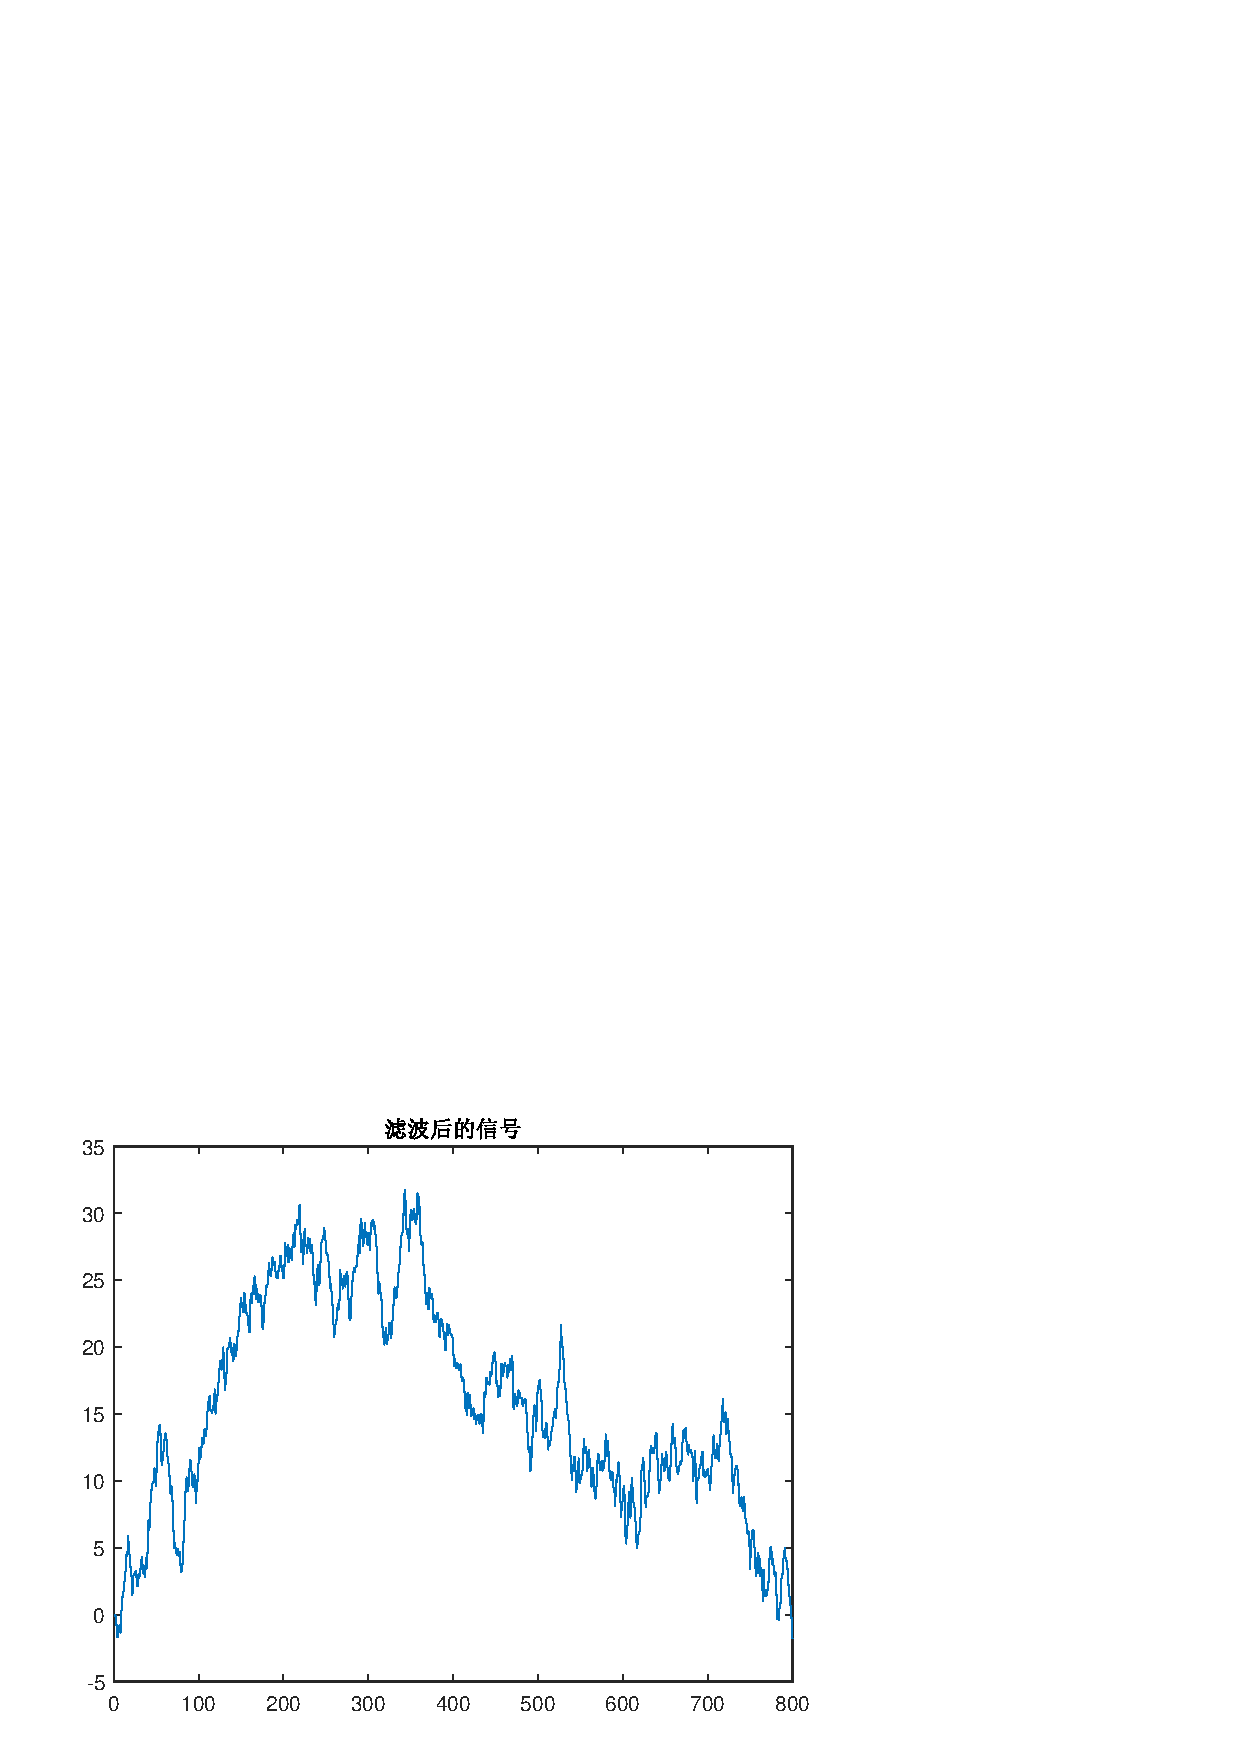
\includegraphics [width=4in]{kalmanfilter_03.png}\\


\end{document}
    
